\documentclass[solution, letterpaper]{cs20inclass}
\usepackage{enumerate}
\usepackage{tikz}
\usepackage{pgf}
\usepackage{tikz}
\usepackage{hyperref}
\begin{document}
\header{19}{Friday, March 11, 2016}

\noindent Author: Crystal Chang, Tom Silver% \\

\paragraph*{Review}

\problem
Let $\{A, B, C, D, E, F, G\}$ be an alphabet of musical notes. A \textbf{song} is defined by some sequence of notes in the alphabet. (So for example, assume only quarter notes on one instrument at one volume is allowed.) For each of the following, state whether the set is finite, countably infinite, or uncountable. Justify your answer by describing a bijection to a set of the same cardinality with known countability.

\begin{enumerate}

\item The set of all songs with exactly 100 notes.
\item The set of all songs with at least 100 notes.
\item The set of all finite length songs.
\item The set of all (possibly infinite length) songs.
\item The set of all (possibly infinite length) songs consisting of only B notes.

\end{enumerate}

\begin{solution}
  % Write your answer here.
\end{solution}

\problem
In the ``Internet Directed Graph'' (IDG), vertices represent webpages, and an arrow from webpage $u$ to webpage $v$ indicates that webpage $u$ contains a hyperlink to webpage $v$. 
\subproblem Is the relation corresponding to the IDG reflexive? Symmetric? Transitive? 
\subproblem What property of a vertex $u$ in the IDG could we use as an estimate for webpage $u$'s popularity? Explain your answer in two sentences or less.
\subproblem Let $Access(u) = \{ v | \text{ there is a path from } u \text{ to } v \text{ in IDG}\}$. Is the following statement true or false? 
\\
\\$Access(u_1) = Access(u_2) \implies u_1 = u_2$. 
\\
\\ If it is true, provide a brief proof. If it is false, provide a counterexample.

\begin{solution}
  % Write your answer here.
\end{solution}

\problem (Bonus) The set of Pythagoras trees:\\
The shape of Pythagoras tree is built by recursively feeding the axiom through the production rules. Each character of the input string is checked against the rule list to determine which character or string to replace it with in the output string. In this example, a '1' in the input string becomes '11' in the output string, while '[' remains the same. 
\begin{itemize}
\item variables: 0,1
\item constants: [,]
\item axiom: 0
\item rules: $(1\rightarrow 11), (0\rightarrow 1[0]0)$
\end{itemize}
\subproblem Give a recursive definition of the  Pythagoras tree.
\subproblem List the first 4 elements.
\subproblem This string can be drawn as an image by using turtle graphics, where each symbol is assigned a graphical operation for the turtle to perform. For example, in the sample above, the turtle may be given the following instructions:
\begin{itemize}
\item 0: draw a line segment ending in a leaf
\item 1: draw a line segment
\item $[$: push position and angle, turn left 45 degrees
\item $]$: pop position and angle, turn right 45 degrees
\end{itemize}
Applying the graphical rules listed above to the earlier recursion, we could get the graphical representation of axiom, 1st and 2nd recursion as the following :\\
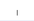
\includegraphics[width=2cm]{0} 
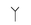
\includegraphics[width=2cm]{1}
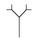
\includegraphics[width=2cm]{2}\\
Draw out the graphical representation of the 3rd and 4th recursion.

\begin{solution}
  % Write your answer here.
\end{solution}




\end{document}
